% ============================================================
%  The Value of Zero
%  Compile with pdfLaTeX (Overleaf default). Standard packages only.
% ============================================================
\documentclass[11pt,a4paper]{article}

\usepackage[T1]{fontenc}
\usepackage[utf8]{inputenc}
\usepackage{lmodern}
\usepackage[margin=25mm]{geometry}
\usepackage{amsmath,amssymb,amsthm}
\usepackage{booktabs}
\usepackage{enumitem}
\usepackage{pgfplots}
\pgfplotsset{compat=1.16}
\usepackage[hidelinks]{hyperref}
\hypersetup{pdftitle={The Value of Zero: A Positional Measure of What a Zero Digit Contributes to a Number},pdfauthor={Sanket Santosh Vidya Manohar},pdfkeywords={zero, place value, positional notation}}

\newtheorem{theorem}{Theorem}
\newtheorem{proposition}{Proposition}
\theoremstyle{definition}
\newtheorem{definition}{Definition}

\newcommand{\Dz}{D}   % number with zeros deleted
\newcommand{\Zv}{Z}   % value of the zeros

% ---------------- Title block ----------------
\title{The Value of Zero: A Positional Measure of What a Zero Digit Contributes to a Number}
\author{%
  Sanket Santosh Vidya Manohar\thanks{ORCID: \url{https://orcid.org/0009-0006-6912-3107}. Website: \url{https://sanketmanohar.com/}. DOI: \url{https://doi.org/10.5281/zenodo.23641598}}\\[2pt]
  \small Independent Researcher, Mumbai, India
}
\date{} % leave empty; arXiv and Zenodo add their own date

\begin{document}
\maketitle

\begin{abstract}
To a layperson the value of zero is simply zero: adding $0$ to any number changes nothing. Yet writing a $0$ after the digit $1$ turns one into ten, and inserting a $0$ into $11$ turns it into $101$. This paper studies that apparent contradiction. We separate the two roles of zero, as a \emph{quantity} (the additive identity) and as a \emph{digit} (a positional placeholder), and we define the value of the zeros in a number $N$ as $N-\Dz(N)$, where $\Dz(N)$ is the number obtained by deleting every zero digit. We derive closed-form formulas for trailing zeros, for a single zero in any position, and a single universal formula valid for any number of zeros in any positions and in any base $b$. We prove that the value of the zeros is always a multiple of $b-1$ (a multiple of $9$ in base ten), show that zeros after a decimal point have negative value, and show that the values of individual zeros are not additive, which we resolve with a sequential rule and with the Shapley value from cooperative game theory. A brief history of zero, from Babylonian placeholders to Brahmagupta's rules, frames the discussion, and we outline uses of the idea in teaching place value. The mathematics rests on standard positional notation; the contribution is the framing, the formulas, and their use as an accessible entry point into place value.
\end{abstract}

\noindent\textbf{Keywords:} zero, place value, positional notation, additive identity, digit deletion, number bases, Shapley value, history of mathematics, mathematics education.

\noindent\textbf{MSC 2020:} 11A63 (radix representation), 01A32 (Indian mathematics), 97F40 (number theory education).

\begin{center}
\begin{minipage}{0.85\textwidth}
\small\itshape
\begin{center}\upshape\bfseries Dedication\end{center}
This paper is for my father. Long before I knew the word ``research'', he would talk with me about quantum physics, about the stars and the shape of the cosmos, and about questions that have no easy answers. He taught me that the lines we are given to think within are only a starting point, and that the most interesting ideas live just beyond them. A question like ``what is the value of zero?'' is exactly the kind of question he taught me to ask. I miss him more than words can hold, and every page of this work carries something of him.
\end{minipage}
\end{center}

% ============================================================
\section{Introduction}

Ask a student ``What is the value of zero?'' and the answer is almost always ``zero''. The answer is correct when zero is used as a quantity: $7+0=7$ and $0+0=0$. It is incomplete when zero is used as a digit. Writing a $0$ after $1$ produces $10$, a number nine larger than $1$; writing two zeros produces $100$, ninety-nine larger. Somehow a symbol worth nothing has changed the number by a great deal.

This paper asks a precise version of the question: \emph{by how much does the presence of zeros change a number, and how much of that change belongs to each zero?} The answer depends on where the zeros stand, how many there are, which digits surround them, and the base of the numeral system. Our aims are to:
\begin{itemize}[nosep]
  \item separate the two roles of zero and explain why adding zero changes nothing while placing it does (Sections~\ref{sec:roles} and~\ref{sec:placing});
  \item give a precise definition of the value of zero in a number (Section~\ref{sec:def});
  \item derive formulas for that value, from simple cases to a universal formula valid in every base, and prove their basic properties (Section~\ref{sec:formulas});
  \item study how the total value can be shared among individual zeros (Section~\ref{sec:attrib}) and what happens after a decimal point (Section~\ref{sec:decimal});
  \item place the topic in its history and discuss its importance and future directions (Sections~\ref{sec:history}, \ref{sec:importance} and~\ref{sec:future}).
\end{itemize}

All results are elementary consequences of positional notation~\cite{ifrah,knuth}. We claim no new deep theorem; instead we offer a concrete, playful measure that makes place value visible and a set of exact formulas a student can verify by hand. Every numerical example in this paper was also checked by computer for all integers below $200{,}000$.

% ============================================================
\section{A Brief History of Zero}\label{sec:history}

\subsection{Zero as a placeholder}
The Babylonians wrote numbers in base sixty. For centuries they left an ambiguous gap where a place was empty. By the Seleucid period (roughly the last three centuries BCE) scribes used a separate mark, two slanted wedges, to show an empty place inside a number~\cite{neugebauer,ifrah}. This was a placeholder only: it was not used at the end of a number and was never treated as a quantity. Greek astronomers, including Ptolemy in the second century CE, used a small circle for empty places in sexagesimal tables~\cite{neugebauer}.

The Maya of Mesoamerica independently developed a positional system (mostly base twenty) with a zero sign, often drawn as a shell, used in their Long Count calendar dates by around the fourth century CE~\cite{kaplan,chrisomalis,joseph}.

\subsection{Zero as a number in India}
In India the decimal place-value system and zero matured together. The Bakhshali manuscript uses a dot for zero; radiocarbon dating reported by the University of Oxford in 2017 placed some of its leaves in the third or fourth century CE, although scholars debate how to interpret these dates~\cite{bodleian,plofker}. In 628~CE Brahmagupta, in the \emph{Br\=ahmasphu\d{t}asiddh\=anta}, became the first known author to treat zero as a number in its own right, stating rules such as: a number plus zero is that number, a number minus zero is that number, and a number times zero is zero~\cite{colebrooke,plofker}. He also attempted to define zero divided by zero as zero, a rule modern mathematics does not accept. An inscription at the Chaturbhuj temple in Gwalior, dated 876~CE, contains one of the oldest securely dated round zero symbols in India~\cite{kaplan,plofker}.

\subsection{Transmission}
The Indian numerals reached the Islamic world, where al-Khw\=arizm\=\i\ wrote on calculation with them around 825~CE~\cite{ifrah}. Leonardo of Pisa (Fibonacci) introduced them to European merchants in \emph{Liber Abaci} in 1202~\cite{sigler}. Over the following centuries the Hindu--Arabic numerals and their zero replaced Roman numerals for calculation, which is the system we use today~\cite{kaplan,seife}.

History therefore already shows the two roles that this paper separates: zero began as a \emph{placeholder} (Babylon, Maya) and only later became a \emph{number} (India).

% ============================================================
\section{The Two Roles of Zero}\label{sec:roles}

\subsection{Zero as a quantity: the additive identity}
As a quantity, zero means ``nothing''. In modern arithmetic its defining property is
\begin{equation}\label{eq:identity}
  a + 0 = 0 + a = a \qquad \text{for every number } a.
\end{equation}
Mathematicians call such an element an \emph{additive identity}. This is not a fact proved from something deeper; it is how zero is defined. In Peano's axioms for the natural numbers, addition is defined by $a+0=a$ and $a+S(b)=S(a+b)$, where $S$ means ``the next number''~\cite{peano}. So the reason adding $0$ changes nothing is that $0$ counts no objects: putting together a collection of $a$ objects and a collection of no objects leaves $a$ objects. Every digit from $1$ to $9$ is a nonzero quantity, so adding it always changes a sum. Zero is the unique number with this property: if $e+a=a$ for even one number $a$, then $e=0$.

\subsection{Zero as a digit: positional notation}
In a positional system with base $b$ ($b=10$ for ordinary numbers), a numeral with digits $d_k d_{k-1}\dots d_1 d_0$, each digit between $0$ and $b-1$ and $d_k\neq 0$, stands for
\begin{equation}\label{eq:positional}
  N = d_k b^k + \dots + d_1 b^1 + d_0 b^0 = \sum_{i=0}^{k} d_i\, b^i .
\end{equation}
We number positions from the right, starting at $0$. In $2030$ the digit $3$ is at position $1$ and the digit $2$ at position $3$. A zero digit contributes $0\cdot b^i=0$ to the sum in~\eqref{eq:positional}, so in this narrow sense zero is still worth nothing. Its real effect is indirect: \textbf{it occupies a position, and this pushes every digit on its left one place higher}, multiplying that digit's contribution by $b$.

% ============================================================
\section{Adding Versus Placing}\label{sec:placing}

Adding and placing are different operations. Writing a digit $d$ to the right of a numeral $N$ (concatenation, written $N\,\|\,d$) gives
\begin{equation}\label{eq:concat}
  N\,\|\,d = b\cdot N + d .
\end{equation}

\begin{proposition}
Appending any digit $d$ to $N$ increases it by $(b-1)N+d$. Appending a zero increases it by exactly $(b-1)N$.
\end{proposition}
\begin{proof}
Subtract $N$ from both sides of~\eqref{eq:concat}.
\end{proof}

So appending a $7$ to $12$ gives $127=10\cdot 12+7$, and appending a $0$ gives $120=10\cdot 12$. \emph{Every} digit causes the ``times $b$'' jump; zero is simply the only digit that adds nothing on top of it, which is why it displays the jump so clearly. Writing a zero on the far left (for example $007$) changes nothing, because no digit lies to its left to be pushed up. These observations answer the question ``why is zero zero when we add it, and not zero when we place it?'': addition combines quantities, while placement shifts positions.

% ============================================================
\section{Defining the Value of Zero}\label{sec:def}

Let $N$ be a positive integer written in base $b$. Let $\Dz(N)$ denote the integer obtained by deleting every zero digit from the numeral of $N$ and reading the remaining digits in order (in base ten this is OEIS sequence A004719~\cite{oeis}).

\begin{definition}[Total value of the zeros]
\begin{equation}\label{eq:def}
  \Zv(N) = N - \Dz(N).
\end{equation}
\end{definition}

\begin{definition}[Marginal value of one zero]
If a zero stands at position $p$, let $N^{(-p)}$ be the number obtained by deleting only that zero. The marginal value of the zero is $N - N^{(-p)}$.
\end{definition}

For example, $\Dz(2030)=23$, so $\Zv(2030)=2007$. A natural first attempt for $101$ is to split it as $1+100$ and say that the zeros turned $1$ into $100$, a change of $99$. Definition~1 instead compares $101$ with $\Dz(101)=11$, giving $\Zv(101)=90$. The difference matters: the split $1+100$ removes a $1$ as well as a $0$, so it measures two changes at once. A precise definition prevents this mixing.

Useful parameters for describing a number are its length $L=k+1$, its number of zeros, the positions of those zeros, and the base. Section~\ref{sec:formulas} shows that length and zero count alone do not determine the value: what matters is, for each nonzero digit, how many zeros stand to its right.

% ============================================================
\section{Formulas for the Value of Zero}\label{sec:formulas}

\subsection{Trailing zeros}
\begin{theorem}\label{thm:trailing}
If $N=M\cdot b^t$, where $M$ has no zero digits (the numeral of $N$ is $M$ followed by $t$ zeros), then
\begin{equation}\label{eq:trailing}
  \Zv(N) = M\,(b^t-1).
\end{equation}
\end{theorem}
\begin{proof}
Here $\Dz(N)=M$, so $\Zv(N)=Mb^t-M$.
\end{proof}
Examples: $\Zv(10)=1\cdot 9=9$; $\Zv(100)=99$; $\Zv(7000)=7\cdot 999=6993$.

\subsection{A single zero in any position}
\begin{theorem}\label{thm:single}
Suppose the numeral of $N$ contains exactly one zero, at position $p$, and let $H$ be the number formed by the digits to the left of that zero. Then
\begin{equation}\label{eq:single}
  \Zv(N) = (b-1)\cdot H\cdot b^{p}.
\end{equation}
\end{theorem}
\begin{proof}
Write $N = H b^{p+1} + 0\cdot b^p + R$, where $R<b^p$ is the part to the right of the zero. Deleting the zero gives $H b^p + R$. The difference is $Hb^{p+1}-Hb^p=(b-1)Hb^p$.
\end{proof}
The digits to the right of the zero do not matter at all. For $101$: $p=1$, $H=1$, so $\Zv=9\cdot 1\cdot 10=90$. For $5073$: $p=2$, $H=5$, so $\Zv=9\cdot 5\cdot 100=4500$, and indeed $5073-573=4500$. Formula~\eqref{eq:single} is also the marginal value of any one zero in a number with several zeros, provided $H$ is read with the other zeros kept in place.

\subsection{The universal formula}
For each nonzero digit $d_i$ let $z_i$ be the number of zero digits to its right, that is, at positions $0,1,\dots,i-1$.

\begin{theorem}[Universal formula]\label{thm:universal}
For every positive integer $N$ in every base $b\ge 2$,
\begin{equation}\label{eq:universal}
  \Zv(N) = \sum_{d_i\neq 0} d_i\, b^{\,i-z_i}\left(b^{z_i}-1\right).
\end{equation}
\end{theorem}
\begin{proof}
When all zeros are deleted, the nonzero digit $d_i$ moves down by exactly $z_i$ places, from position $i$ to position $i-z_i$, and the order of the nonzero digits is unchanged. Hence $N=\sum d_i b^i$ and $\Dz(N)=\sum d_i b^{\,i-z_i}$, both sums over nonzero digits. Subtracting term by term gives~\eqref{eq:universal}.
\end{proof}

Theorems~\ref{thm:trailing} and~\ref{thm:single} are special cases. In words: \textbf{the value of the zeros is the total amount by which they lift the nonzero digits on their left.} Example, $2030$ in base ten: the $3$ (position $1$) has one zero to its right and contributes $3\cdot 10^0\cdot 9=27$; the $2$ (position $3$) has two zeros to its right and contributes $2\cdot 10^1\cdot 99=1980$. The total, $2007$, equals $2030-23$. Example in base two: $1010_2$ (ten) becomes $11_2$ (three) when its zeros are deleted, so its zeros are worth $7$, and~\eqref{eq:universal} gives $1\cdot 2^1(2^2-1)+1\cdot 2^0(2^1-1)=6+1=7$.

\subsection{Properties}
\begin{theorem}[Divisibility]\label{thm:div}
For every $N$, $\Zv(N)$ is a multiple of $b-1$. In base ten, the value of the zeros is always a multiple of $9$.
\end{theorem}
\begin{proof}
Each term of~\eqref{eq:universal} contains the factor $b^{z}-1=(b-1)(b^{z-1}+\dots+b+1)$. Alternatively: $N$ and $\Dz(N)$ have the same digit sum, and a number is congruent to its digit sum modulo $b-1$, so $N\equiv \Dz(N)\pmod{b-1}$.
\end{proof}
Theorem~\ref{thm:div} connects the value of zero to the classical check called \emph{casting out nines}: $9$, $90$, $990$, $2007=9\cdot 223$ and $6993=9\cdot 777$ are all multiples of $9$.

\begin{theorem}[Basic bounds]
$0\le \Zv(N)<N$, with $\Zv(N)=0$ exactly when $N$ has no zero digit.
\end{theorem}
\begin{proof}
Every term of~\eqref{eq:universal} is nonnegative, and a term is positive exactly when some zero lies to the right of a nonzero digit, which happens whenever the numeral contains a zero (the leading digit is nonzero). Since $\Dz(N)\ge 1$, $\Zv(N)<N$.
\end{proof}

\begin{proposition}
The length of $N$ and the number of its zeros do not determine $\Zv(N)$.
\end{proposition}
\begin{proof}
$1001$ and $1100$ both have length $4$ and two zeros, but $\Zv(1001)=1001-11=990$ and $\Zv(1100)=1100-11=1089$.
\end{proof}
So no formula using only length and zero count can work; the positions of the zeros relative to the nonzero digits are essential, exactly as~\eqref{eq:universal} shows. One formula nonetheless covers every case, so there is no need for a separate formula for each situation.

% ============================================================
\section{How Much Is Each Zero Worth?}\label{sec:attrib}

A tempting idea is to give each zero its marginal value (Definition~2) and add them up. This fails. In $2030$, deleting only the last zero gives $203$, a drop of $1827$; deleting only the middle zero gives $230$, a drop of $1800$. Their sum, $3627$, exceeds $\Zv(2030)=2007$. Zeros reinforce each other: each one raises the position of the other's left-hand neighbours, so their effects overlap.

\begin{proposition}
Marginal values of zeros are not additive in general: their sum can exceed $\Zv(N)$.
\end{proposition}

\subsection{Sequential attribution}
Rebuild $N$ from $\Dz(N)$ by inserting its zeros one at a time in a fixed order, and credit each zero with the jump it causes. The credits always add up to $\Zv(N)$, but they depend on the order. For $2030$, inserting the last zero first gives $23\to 230$ (credit $207$), then $230\to 2030$ (credit $1800$); inserting the middle zero first gives $23\to 203$ (credit $180$), then $203\to 2030$ (credit $1827$).

\subsection{Fair attribution with the Shapley value}
The order-dependence can be removed by averaging the credit of each zero over all possible insertion orders. This is precisely the Shapley value of cooperative game theory~\cite{shapley}, with the zeros as players and $\Zv$ as the worth of a coalition. It always adds up to $\Zv(N)$, treats identical situations identically, and gives each zero its average contribution.

\begin{table}[ht]
\centering\small
\begin{tabular}{@{}cl ccc@{}}
\toprule
Number & Zero & Credit if first & Credit if second & Shapley value \\
\midrule
2030 & middle (position 2) & 180 & 1800 & 990 \\
2030 & last (position 0)   & 207 & 1827 & 1017 \\
1005 & position 2          & 90  & 900  & 495 \\
1005 & position 1          & 90  & 900  & 495 \\
\bottomrule
\end{tabular}
\caption{Attribution of the total value of the zeros among individual zeros. Shapley values sum to $\Zv(2030)=2007$ and $\Zv(1005)=990$.}
\label{tab:shapley}
\end{table}

In $1005$ the two zeros play symmetric roles, so each receives half of $990$. Finding a simple closed formula for the Shapley value of each zero in a general number is, to our knowledge, an open and pleasant exercise (Section~\ref{sec:future}).

% ============================================================
\section{Zeros After the Decimal Point}\label{sec:decimal}

Definition~1 extends to decimals: delete zero digits and compare. Leading zeros of the integer part ($0.5$ versus $.5$, or $007$ versus $7$) and trailing zeros of the fractional part ($2.50$ versus $2.5$) are worth exactly $0$. A zero placed between the decimal point and a later nonzero digit, however, pushes the digits on its \emph{right} to smaller places, so its value is negative.

\begin{theorem}\label{thm:decimal}
Let a zero stand at the $j$-th place after the point, and let $T$ be the value of all digits to its right (as part of the original number). Deleting this zero changes the number by
\begin{equation}\label{eq:decimal}
  \text{value of the zero} = -(b-1)\cdot T .
\end{equation}
\end{theorem}
\begin{proof}
Deleting the zero moves every digit to its right one place towards the point, multiplying their combined value $T$ by $b$. The number therefore changes from $x$ to $x+(b-1)T$, so the zero was worth $T-bT=-(b-1)T$.
\end{proof}
Example: in $0.05$, $T=0.05$, so the zero is worth $-9\cdot 0.05=-0.45$, and indeed $0.05-0.5=-0.45$.

Formulas~\eqref{eq:single} and~\eqref{eq:decimal} mirror each other: a zero \emph{left} of the point is worth $(b-1)$ times the part it lifts, and a zero \emph{right} of the point is worth minus $(b-1)$ times the part it pushes down. Zeros make numbers larger on one side of the point and smaller on the other.

% ============================================================
\section{Worked Examples and Patterns}\label{sec:examples}

\begin{table}[ht]
\centering\small
\begin{tabular}{@{}rrrrl@{}}
\toprule
$N$ & Zeros deleted, $\Dz(N)$ & Value of zeros, $\Zv(N)$ & $\Zv(N)/9$ & Formula used \\
\midrule
10 & 1 & 9 & 1 & Theorem 1 \\
100 & 1 & 99 & 11 & Theorem 1 \\
101 & 11 & 90 & 10 & Theorem 2 \\
1{,}001 & 11 & 990 & 110 & Theorem 3 \\
1{,}005 & 15 & 990 & 110 & Theorem 3 \\
1{,}100 & 11 & 1{,}089 & 121 & Theorems 1, 3 \\
2{,}030 & 23 & 2{,}007 & 223 & Theorem 3 \\
5{,}073 & 573 & 4{,}500 & 500 & Theorem 2 \\
7{,}000 & 7 & 6{,}993 & 777 & Theorem 1 \\
10{,}203 & 123 & 10{,}080 & 1{,}120 & Theorem 3 \\
\bottomrule
\end{tabular}
\caption{Values of the zeros for selected base-ten numbers. Every value is a multiple of $9$ (Theorem~\ref{thm:div}).}
\label{tab:examples}
\end{table}

\paragraph{A large example.} Take $N=1{,}002{,}030{,}400$, which has six zeros. Deleting them leaves $\Dz(N)=1234$, so $\Zv(N)=1{,}002{,}029{,}166=9\cdot 111{,}336{,}574$. By~\eqref{eq:universal}, the four nonzero digits are lifted by $396$ (the $4$), $29{,}970$ (the $3$), $1{,}999{,}800$ (the $2$) and $999{,}999{,}000$ (the $1$), which sum to the same total.

\begin{figure}[ht]
\centering
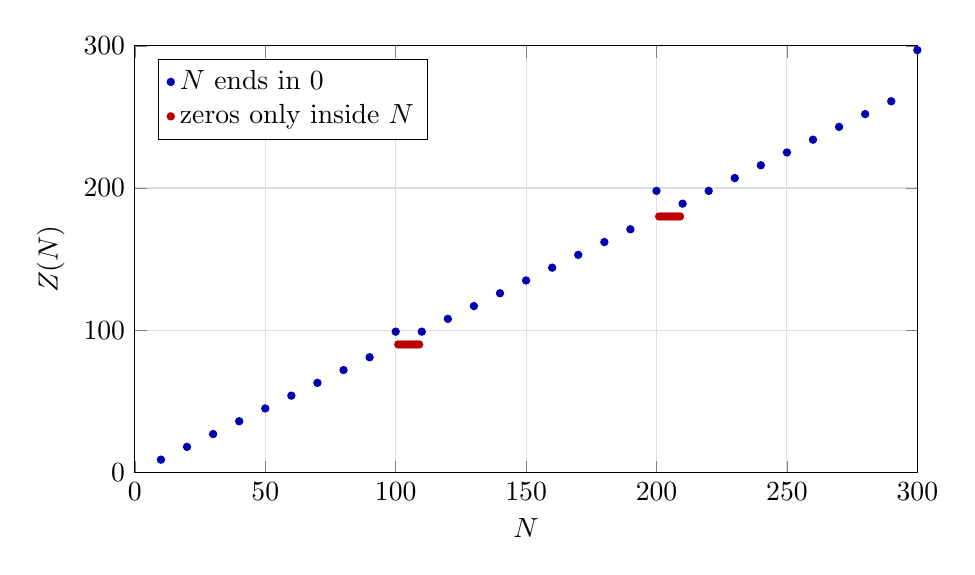
\begin{tikzpicture}
\begin{axis}[
  width=0.95\textwidth, height=7cm,
  xmin=0, xmax=300, ymin=0, ymax=300,
  xlabel={$N$}, ylabel={$\Zv(N)$},
  grid=major, grid style={gray!25},
  legend pos=north west, legend cell align=left,
  mark size=1.3pt]
\addplot[only marks, mark=*, blue!70!black] coordinates {(10,9) (20,18) (30,27) (40,36) (50,45) (60,54) (70,63) (80,72) (90,81) (100,99) (110,99) (120,108) (130,117) (140,126) (150,135) (160,144) (170,153) (180,162) (190,171) (200,198) (210,189) (220,198) (230,207) (240,216) (250,225) (260,234) (270,243) (280,252) (290,261) (300,297)};
\addlegendentry{$N$ ends in $0$}
\addplot[only marks, mark=*, red!75!black] coordinates {(101,90) (102,90) (103,90) (104,90) (105,90) (106,90) (107,90) (108,90) (109,90) (201,180) (202,180) (203,180) (204,180) (205,180) (206,180) (207,180) (208,180) (209,180)};
\addlegendentry{zeros only inside $N$}
\end{axis}
\end{tikzpicture}
\caption{The value of the zeros $\Zv(N)$ for $N=1$ to $300$ (numbers with no zero, where $\Zv=0$, are omitted). Numbers ending in $0$ lie close to the line $\Zv=0.9N$ because appending a zero multiplies by ten ($100$, $200$ and $300$ sit slightly higher, at $0.99N$). Numbers with an inner zero form short flat runs: $101$ to $109$ are all worth $90$ and $201$ to $209$ are all worth $180$, because by Theorem~\ref{thm:single} the value depends only on the digits to the left of the zero.}
\label{fig:plot}
\end{figure}

Two patterns are visible. First, for a number ending in $t$ zeros, $\Zv(N)/N=1-10^{-t}$, so a single trailing zero accounts for $90\%$ of the number, two for $99\%$, and three for $99.9\%$. Second, three-digit numbers with a middle zero all have the value $90\cdot H$, where $H$ is the first digit, regardless of the last digit: $101$ through $109$ are all worth $90$.

% ============================================================
\section{Why the Value of Zero Matters}\label{sec:importance}

\paragraph{Place value in teaching.} Place value is among the most important and most frequently misunderstood ideas in primary mathematics; Ma's comparative study of teachers highlights how much depends on understanding it deeply~\cite{ma}. Asking ``what is this zero worth?'' turns the abstract rule~\eqref{eq:positional} into a concrete calculation that students can do by deleting a digit and subtracting. The $101$ example, where an intuitive answer ($99$) differs from the precise one ($90$), makes a natural classroom discussion.

\paragraph{Computing.} Every digital computer stores numbers in base two, where the digits are only $0$ and $1$. In binary, Theorem~\ref{thm:universal} applies with $b=2$ and every zero contributes by lifting the ones on its left. The IEEE~754 standard for floating-point arithmetic even distinguishes a positive and a negative zero, which behave identically under addition yet carry information under division and in limits~\cite{ieee754}.

\paragraph{Mathematics.} Zero underlies the empty set, the origin of coordinates, the idea of a limit approaching zero, and the rule that division by zero is undefined. Its arrival in India as a full number made modern algebra possible~\cite{kaplan,plofker}.

% ============================================================
\section{Limitations and Future Scope}\label{sec:future}

The formulas in this paper follow directly from positional notation and are well within classical number theory; their contribution is a new framing rather than new mathematics. Within that framing several directions remain open:
\begin{itemize}[nosep]
  \item \textbf{Closed form for fair shares.} Find a simple formula for the Shapley value of each zero (Section~\ref{sec:attrib}) in terms of positions and digits.
  \item \textbf{Integer sequences.} Check whether the sequence $\Zv(N)=N-\Dz(N)$ ($9$ at $N=10$, $18$ at $N=20$, and so on) and its base-$b$ versions are recorded in the OEIS~\cite{oeis} and, if not, submit them.
  \item \textbf{Averages and growth.} Study the average value of $\Zv(N)/N$ over all $L$-digit numbers, and how it behaves as $L$ grows.
  \item \textbf{Other notations.} Compare with systems that lack a zero (Roman numerals, bijective base ten), where the question cannot even be asked.
  \item \textbf{Classroom study.} Use the value-of-zero activity with students and measure whether it improves understanding of place value compared with standard instruction.
\end{itemize}

% ============================================================
\section{Conclusion}

Zero is worth nothing as a quantity and a great deal as a digit. Separating these roles explains why $7+0=7$ while $1$ followed by $0$ is $10$: addition combines quantities, but placing a digit shifts positions. Defining the value of the zeros in $N$ as $N-\Dz(N)$ gives a single universal formula~\eqref{eq:universal}, valid for any number of zeros in any positions and any base, from which formulas for trailing and single zeros follow. The value is always a multiple of $b-1$, is negative for zeros just after a decimal point, and cannot simply be split zero by zero, although the Shapley value gives a fair division. We hope the question ``what is the value of zero?'' serves as a small spark for students meeting place value for the first time.

\section*{Acknowledgement}
I am deeply grateful to my father, my first and finest teacher. His conversations about quantum physics and the cosmos taught me to look past the obvious answer and to keep asking ``why?''. That habit of mind is the true origin of this paper, and I thank him for it with all my heart.

% ============================================================
\begin{thebibliography}{99}

\bibitem{kaplan} R.~Kaplan, \emph{The Nothing That Is: A Natural History of Zero}. New York, NY, USA: Oxford University Press, 1999.

\bibitem{seife} C.~Seife, \emph{Zero: The Biography of a Dangerous Idea}. New York, NY, USA: Viking, 2000.

\bibitem{ifrah} G.~Ifrah, \emph{The Universal History of Numbers: From Prehistory to the Invention of the Computer}. New York, NY, USA: Wiley, 2000.

\bibitem{joseph} G.~G.~Joseph, \emph{The Crest of the Peacock: Non-European Roots of Mathematics}, 3rd ed. Princeton, NJ, USA: Princeton University Press, 2011.

\bibitem{colebrooke} H.~T.~Colebrooke, Trans., \emph{Algebra, with Arithmetic and Mensuration, from the Sanscrit of Brahmegupta and Bh\'ascara}. London, U.K.: John Murray, 1817.

\bibitem{neugebauer} O.~Neugebauer, \emph{The Exact Sciences in Antiquity}, 2nd ed. Providence, RI, USA: Brown University Press, 1957.

\bibitem{plofker} K.~Plofker, \emph{Mathematics in India}. Princeton, NJ, USA: Princeton University Press, 2009.

\bibitem{sigler} L.~E.~Sigler, \emph{Fibonacci's Liber Abaci: A Translation into Modern English of Leonardo Pisano's Book of Calculation}. New York, NY, USA: Springer, 2002.

\bibitem{shapley} L.~S.~Shapley, ``A value for $n$-person games,'' in \emph{Contributions to the Theory of Games II}, H.~W.~Kuhn and A.~W.~Tucker, Eds. Princeton, NJ, USA: Princeton University Press, 1953, pp.~307--317.

\bibitem{ieee754} \emph{IEEE Standard for Floating-Point Arithmetic}, IEEE Std 754-2019, 2019.

\bibitem{oeis} OEIS Foundation Inc., ``Sequence A004719: Delete all 0's from $n$,'' \emph{The On-Line Encyclopedia of Integer Sequences}. [Online]. Available: \url{https://oeis.org/A004719}

\bibitem{knuth} D.~E.~Knuth, \emph{The Art of Computer Programming, Vol.~2: Seminumerical Algorithms}, 3rd ed. Reading, MA, USA: Addison-Wesley, 1997, Sec.~4.1.

\bibitem{bodleian} Bodleian Libraries, University of Oxford, ``Carbon dating finds Bakhshali manuscript contains oldest recorded origins of the symbol `zero','' press release, 14~Sept.~2017. [Online]. Available: \url{https://www.glam.ox.ac.uk/node/218481}

\bibitem{peano} G.~Peano, \emph{Arithmetices Principia, Nova Methodo Exposita}. Turin, Italy: Fratres Bocca, 1889.

\bibitem{chrisomalis} S.~Chrisomalis, \emph{Numerical Notation: A Comparative History}. Cambridge, U.K.: Cambridge University Press, 2010.

\bibitem{ma} L.~Ma, \emph{Knowing and Teaching Elementary Mathematics: Teachers' Understanding of Fundamental Mathematics in China and the United States}. Mahwah, NJ, USA: Lawrence Erlbaum Associates, 1999.

\end{thebibliography}

\end{document}
